\providecommand{\main}{../../../..}
\documentclass[\main/dresen_thesis.tex]{subfiles}
\begin{document}
  \label{sec:looselyPackedNS:nanoparticle:sas}
  Small-angle X-ray scattering measured at GALAXI (\refsec{ch:lss:galaxi}) and small-angle neutron scattering measured at D33 (\refsec{ch:lss:d33}) was performed to quantitatively characterize the nanoparticle dispersions.
  The azimuthally averaged data is shown in \reffig{fig:looselyPackedNP:nanoparticle:sas}.
  From the qualitative comparison of the data, it is visible that the first form factor minima appears for IOS-11 at smaller $q$ values than for IOS-7 and that the minima of IOS-11 are sharper.
  The smaller $q$ value of the scattering vector translates to a larger particle size and the sharper minima to a smaller size distribution.
  Both observations are in agreement with the observations from TEM (\refsec{sec:looselyPackedNS:nanoparticle:tem}).

  \paragraphNewLine{Determination of Particle Sizes And Core-Shell Structure with SAS}

    To determine the size of the particles, the data for both samples and both experiments is fitted to a form factor of spherical particles with an additional oleic acid surfactant shell dispersed in cyclohexane.
    The best fit is shown in \reffig{fig:looselyPackedNP:nanoparticle:sas}, where the scattering length density profile is in each case shown in the insets.
    In all cases, the SLD of the core is fixed to the value of magnetite.
    Furthermore the SLD of oleic acid and the solvents, cyclohexane for SAXS and toluene-$\mathit{d8}$ for SANS respectively, are fixed.
    Additionally, a spherical form factor describing free oleic acid micelles in the dispersion is added incoherently to the SANS model.
    The parameters of the form factors are given in \reftab{tab:looselyPackedNP:nanoparticle:sas}.

    For IOS-11 the spherical form factor with a surfactant shell shows a small deviation for small $q$ values.
    This is attributed to a too high particle concentration in the dispersion, which results in a structure factor for small $q$.
    For larger $q$ values the structure factor is however negligible and therefore the data can still be well described by the form factor.
    The particle diameter of $10.580(2) \unit{nm}$ and size distribution of $5.59(3) \%$ determined by SAXS is fixed in the SANS form factor to determine then the surfactant shell thickness of $1.47(4)$, which is also implemented in the SAXS form factor for self-consistency.
    The instrumental resolution is fixed to $1.7 \unit{mrad}$ and $2.8 \unit{mrad}$ for the angular resolution at large and short sample-to-detector distance respectively, and to $10 \%$ (FWHM) in wavelength resolution.
    From the number density a particle concentration of $17.3(1) \unit{mg \, mL^{-1}}$ in SAXS and $1.8(1) \unit{mg \, mL^{-1}}$ in SANS.
    The volume concentration of oleic acid in the dispersion is determined to $1.1(1) \cdot 10^{-4}$.

    For IOS-7, the same spherical form factor with a surfactant shell is used.
    For simplicity, the second mode observed in TEM (\refsec{sec:looselyPackedNS:nanoparticle:tem}) is neglected.
    The obtained particle diameter is $6.98(1) \unit{nm}$ with a size distribution of $9.6(2) \unit{\%}$.
    Due to the relatively broad size distribution and small size of the nanoparticles resulting in only one visible form factor minima, the SANS data is not highly sensitive to the size of the surfactant shell thickness.
    As the particle concentration, shell thickness and later the particle magnetization from SANSPOL are highly correlated parameters, the shell thickness is fixed to the same value as observed for IOS-11 with $1.47 \unit{nm}$ to be in a comparable order of magnitude.
    The particle concentration in SAXS corresponds to $3.8(1) \unit{mg \, mL^{-1}}$ and in SANS to $0.84(1) \unit{mg \, mL^{-1}}$, the volume concentration of the oleic acid micelles to $1.63(4) \unit{\cdot 10^{-4}}$.

    \begin{figure}[!htbp]
      \centering
      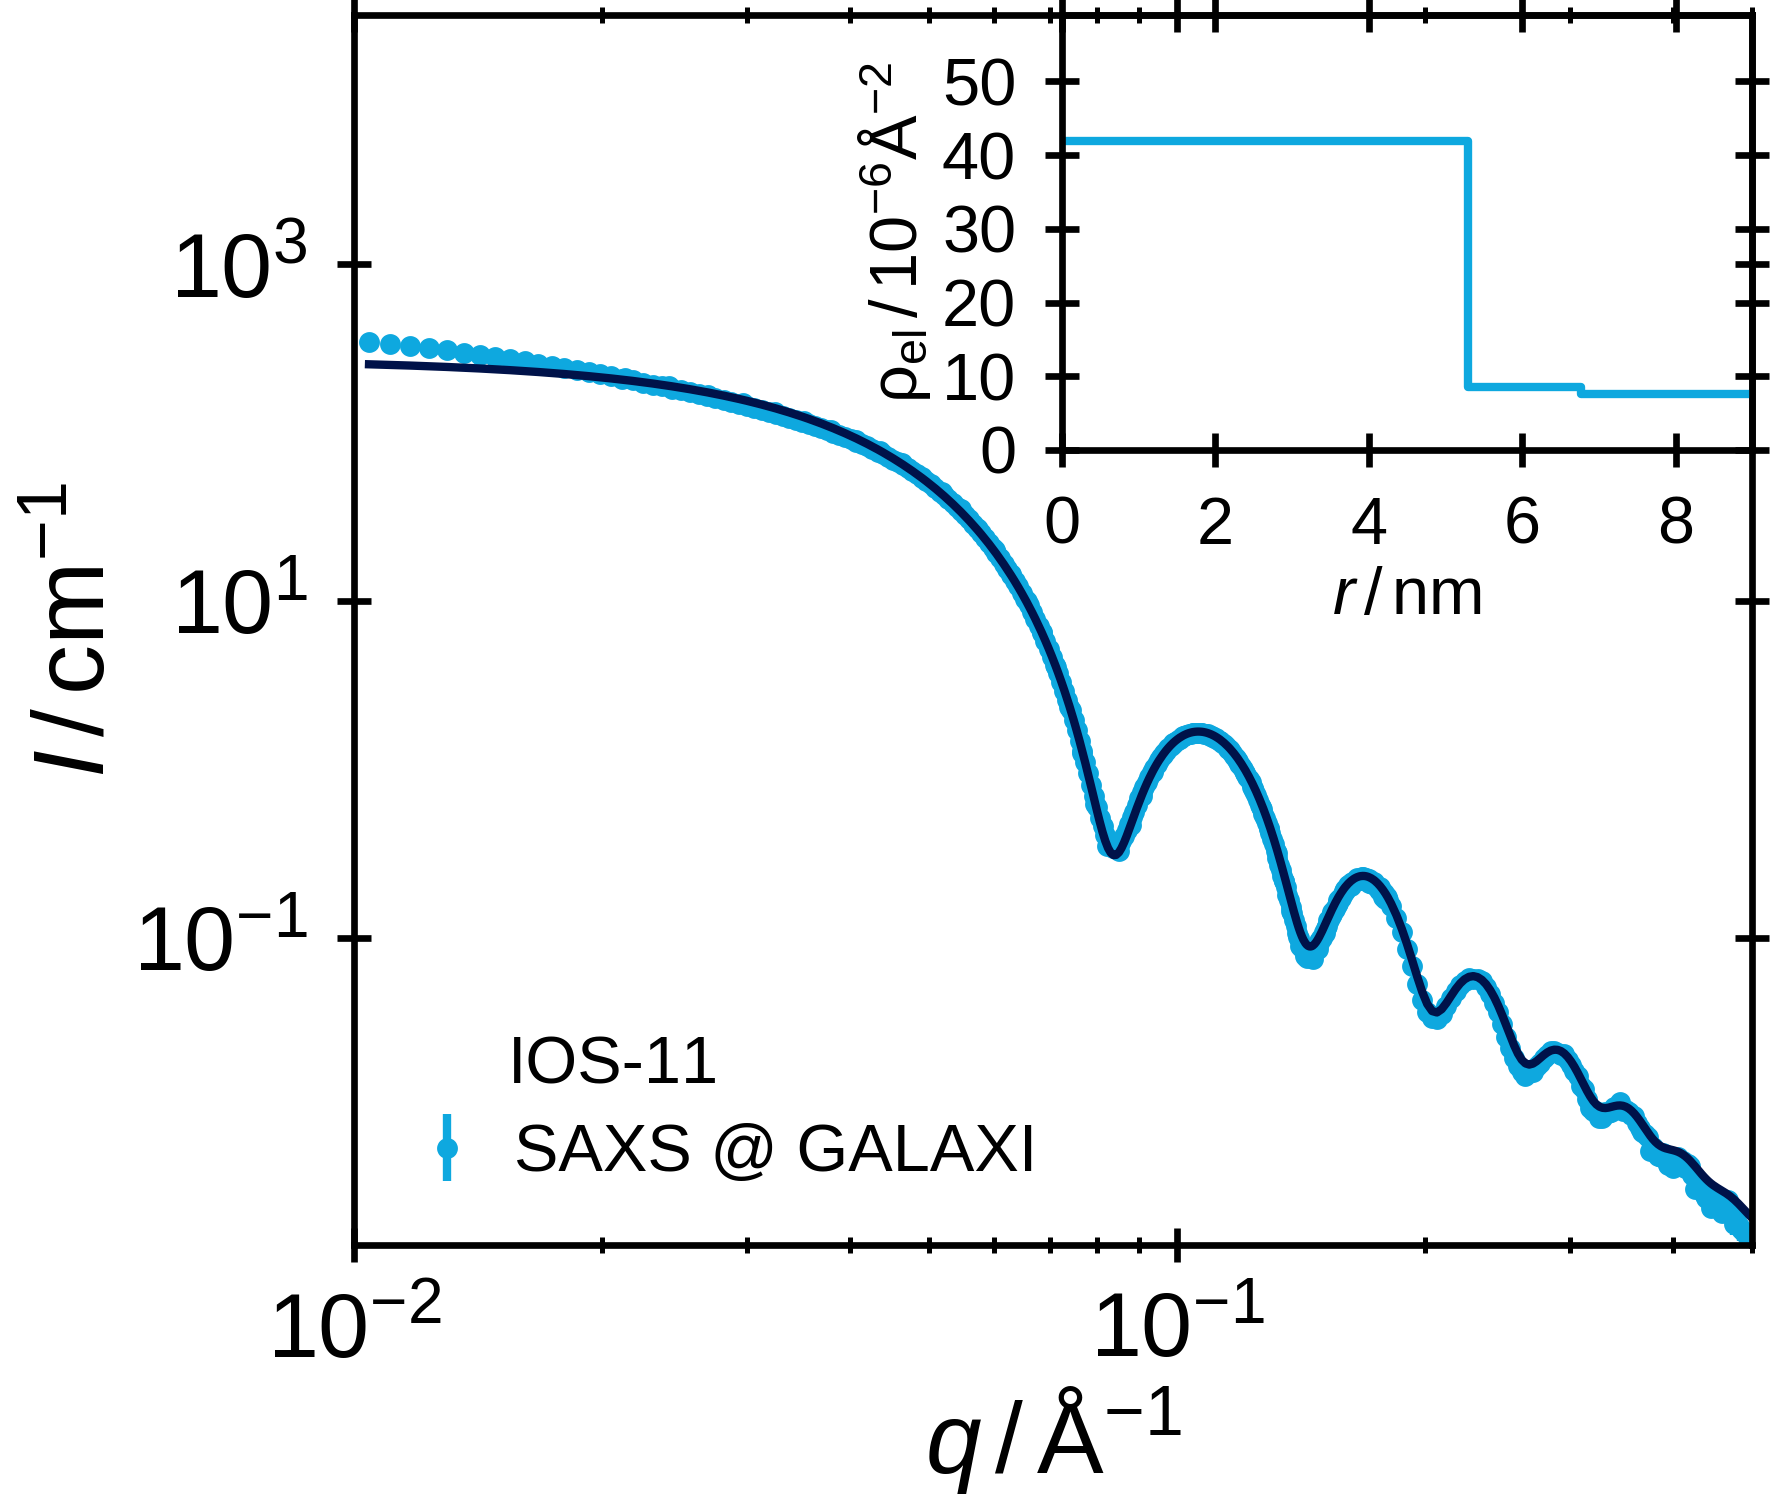
\includegraphics{looselyPackedNP_SAS_IOS-11_SAXS}
      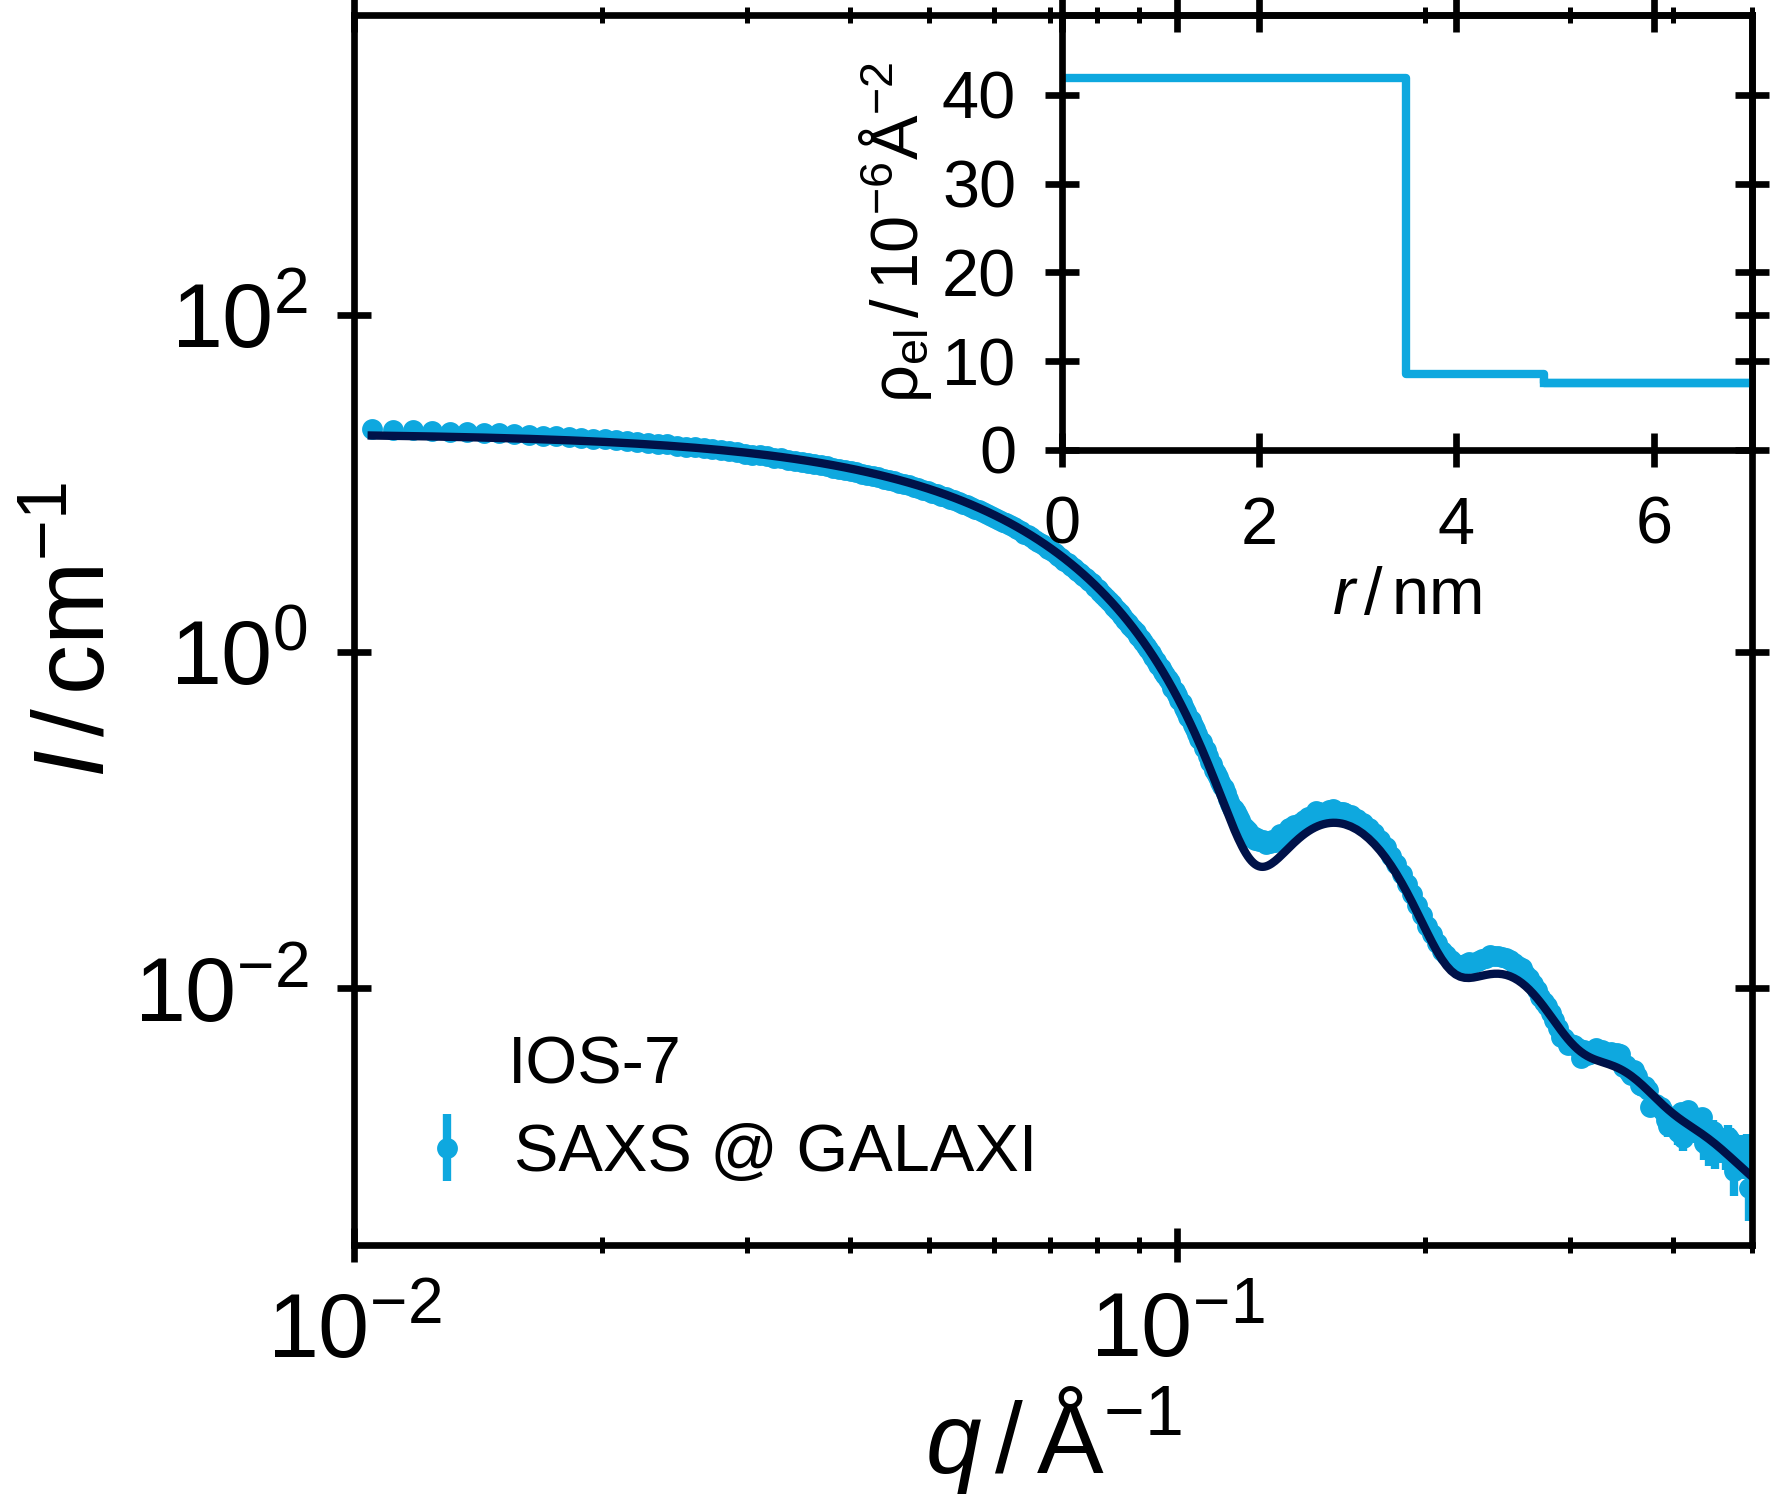
\includegraphics{looselyPackedNP_SAS_IOS-7_SAXS}
      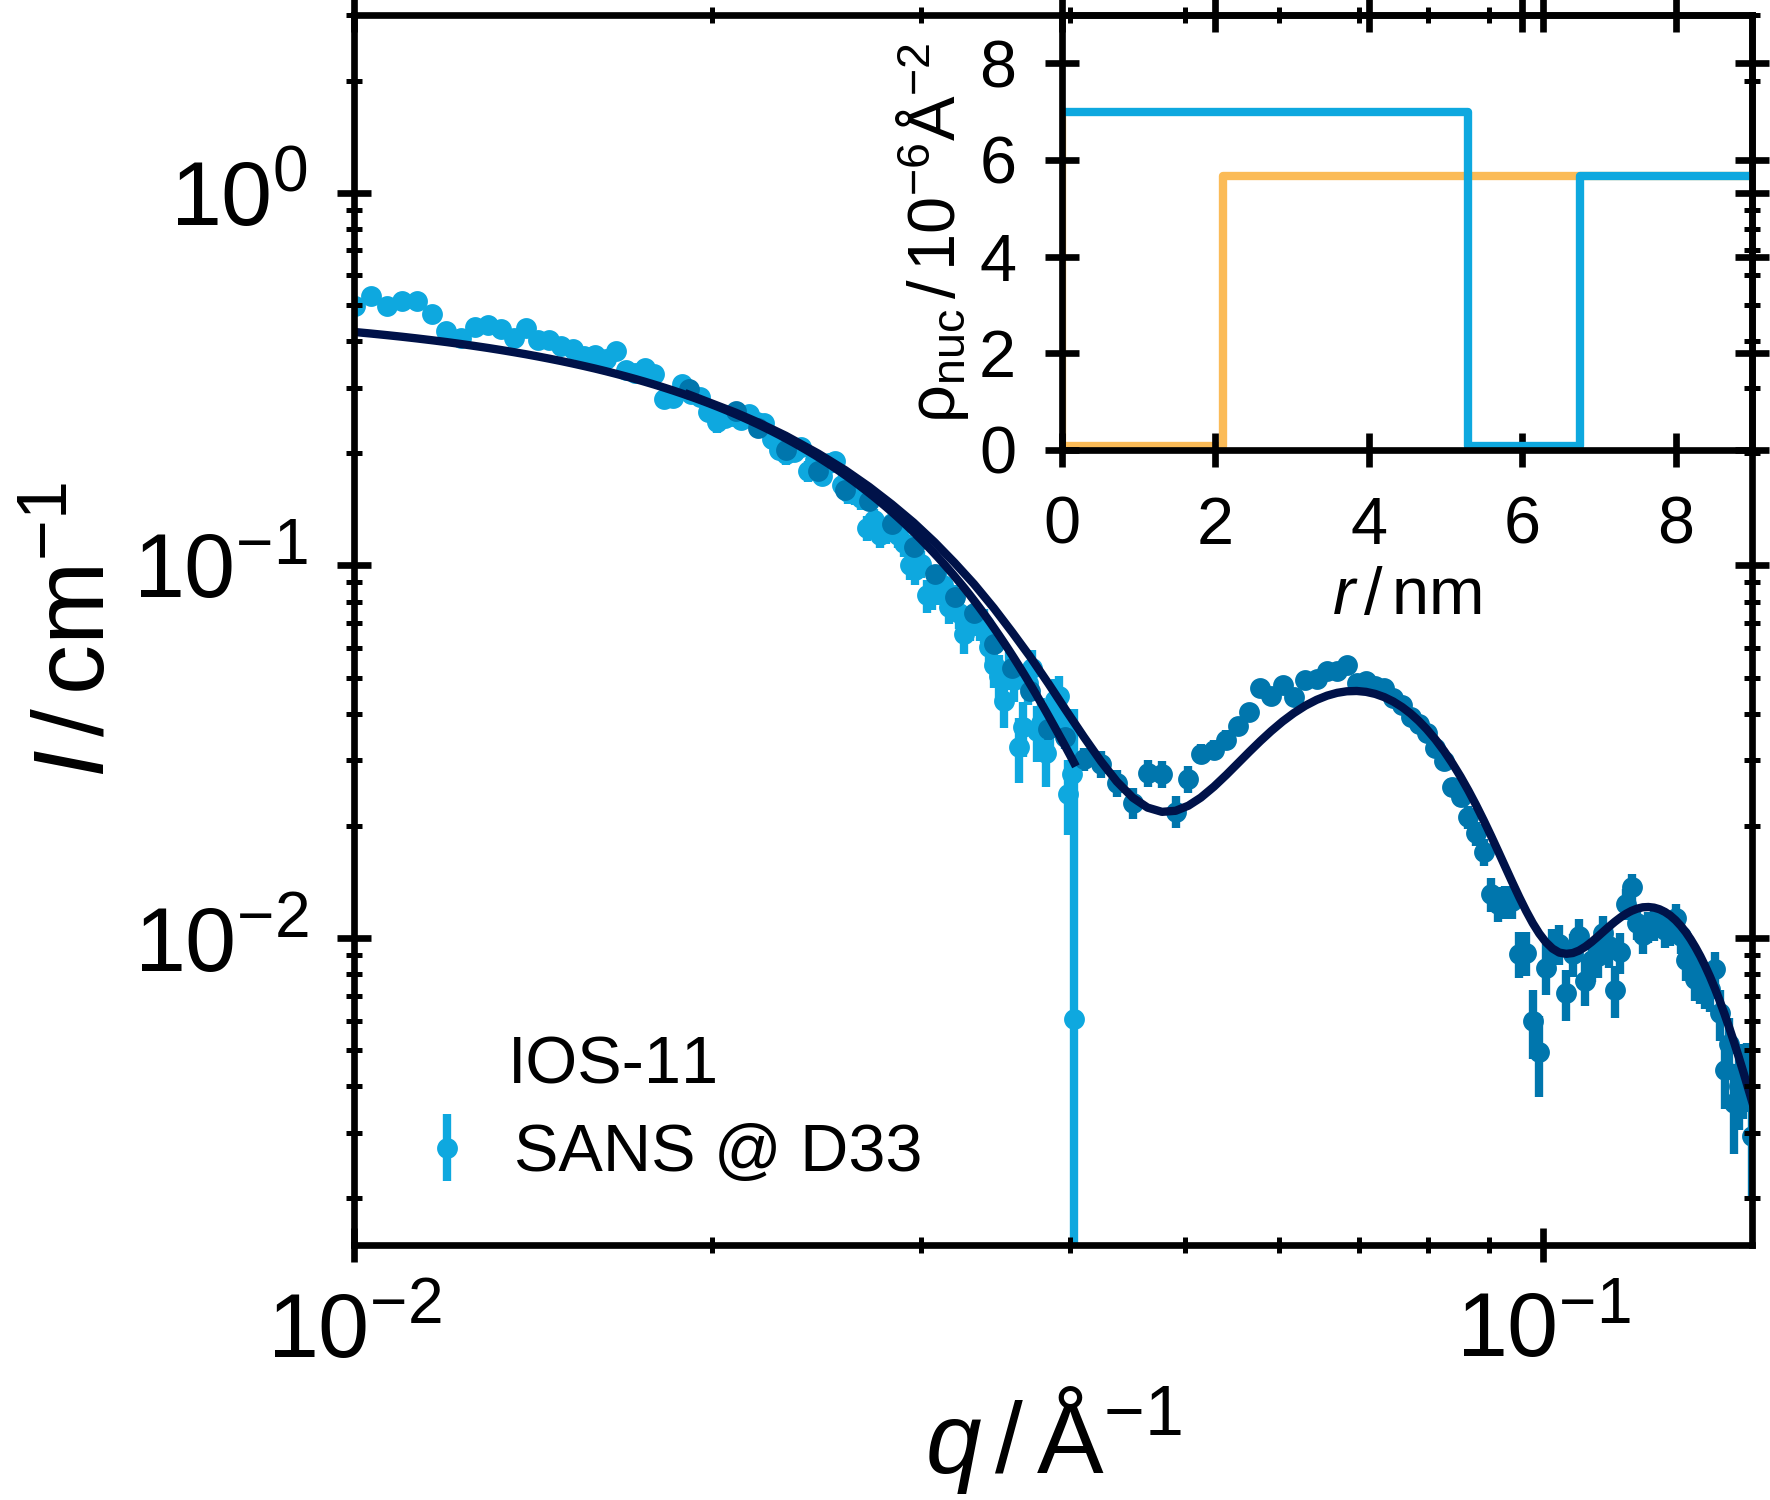
\includegraphics{looselyPackedNP_SAS_IOS-11_SANS}
      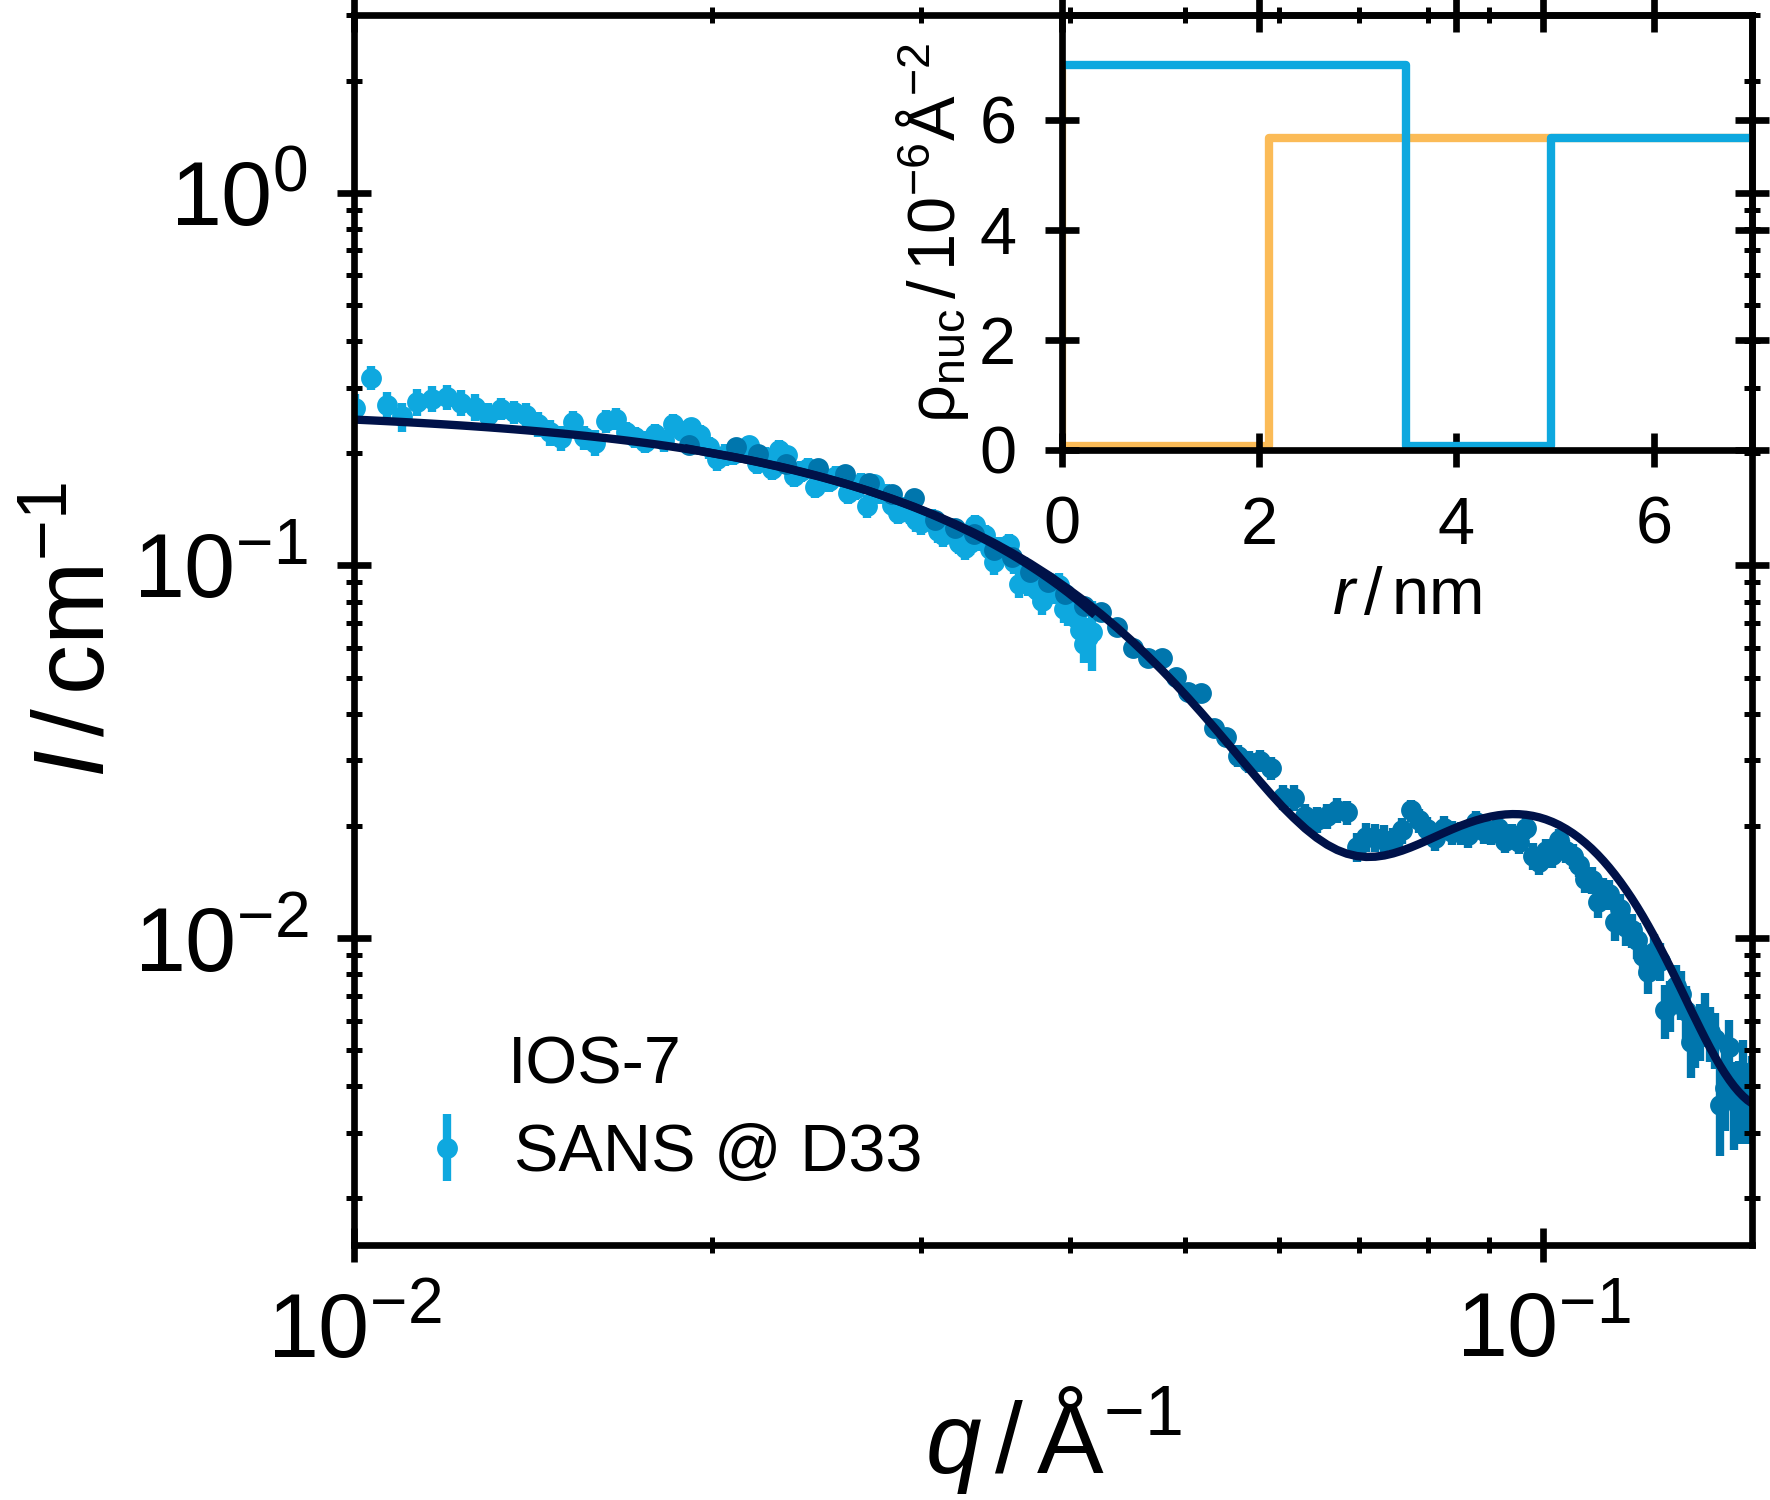
\includegraphics{looselyPackedNP_SAS_IOS-7_SANS}
      \caption{\label{fig:looselyPackedNP:nanoparticle:sas}Small-angle X-ray (upper) and neutron (lower) scattering for IOS-11 (left) and IOS-7 (right). The X-ray and neutron data sets are fitted to a spherical core-shell-surfactant form factor to estimate the average particle size, thickness of the two phases and the surfactant shell thickness, which are visible in the SLD profile insets. Additionally the particle size distribution is obtained and in the case of IOS-7 two modes are needed to describe the data properly (shown by two SLD profiles in the inset).}
    \end{figure}

    \begin{table}[!htbp]
      \centering
      \caption{\label{tab:looselyPackedNP:nanoparticle:sas}Parameters for the spherical model of IOS-11 and IOS-7.}
      \begin{tabular}{ c | l | l }
        \rule{0pt}{2ex} \textbf{SAXS}  & \textbf{IOS-11} & \textbf{IOS-7} \\
        \hline
        \rule{0pt}{2ex} $R \, / \unit{nm}$                                                  & $5.290(1)$           & $3.488(7)$\\
        \rule{0pt}{2ex} $\sigma_{R}\, / \unit{\%}$                                          & $5.59(3)$            & $9.6(2)$ \\
        \rule{0pt}{2ex} $n \, / \unit{10^{-8} \angstrom^{-3}}$                              & $0.5331(7)$          & $0.411(2)$\\
        \hline
        \rule{0pt}{2ex} $\rho_\mathrm{magnetite} \, / \unit{10^{-6} \angstrom^{-2}}$        & \multicolumn{2}{c}{$41.85$}\\
        \rule{0pt}{2ex} $\rho_\mathrm{oleic\, acid} \, / \unit{10^{-6} \angstrom^{-2}}$     & \multicolumn{2}{c}{$8.52$}\\
        \rule{0pt}{2ex} $\rho_\mathrm{cyclohexane} \, / \unit{10^{-6} \angstrom^{-2}}$      & \multicolumn{2}{c}{$7.55$}\\
        \hline
        \rule{0pt}{2ex} $c_m \, / \unit{mg\, mL^{-1}}$                                      & $17.3(1)$            & $3.8(1)$\\
        \hline
        \rule{0pt}{2ex} $\chi^2$                                                            & $73.0$               & $133.5$\\
        \hline
        \hline
        \rule{0pt}{2ex} \textbf{SANS} \\
        \hline
        \rule{0pt}{2ex} $D_{\mathrm{oleic \, acid}, \, 2}\, / \unit{nm}$                    & $1.47(4)$            & $1.47$    \\
        \rule{0pt}{2ex} $n_\mathrm{NP} \, / \unit{10^{-8} \angstrom^{-3}}$                  & $0.056(6)$           & $0.090(1)$\\
        \rule{0pt}{2ex} $r_\mathrm{OA} / \unit{nm}$                                         & $2.1$                & $2.1$ \\
        \rule{0pt}{2ex} $n_\mathrm{OA} \, / \unit{10^{-8} \angstrom^{-3}}$                  & $0.28(3)$            & $0.42(1)$  \\
        \hline
        \rule{0pt}{2ex} $\rho_\mathrm{magnetite} \, / \unit{10^{-6} \angstrom^{-2}}$        & \multicolumn{2}{c}{$7.00$}\\
        \rule{0pt}{2ex} $\rho_\mathrm{oleic \, acid} \, / \unit{10^{-6} \angstrom^{-2}}$    & \multicolumn{2}{c}{$0.078$}\\
        \rule{0pt}{2ex} $\rho_{\mathrm{toluene-}d8} \, / \unit{10^{-6} \angstrom^{-2}}$     & \multicolumn{2}{c}{$5.66$}\\
        \rule{0pt}{2ex} $\lambda^\mathrm{sans} \, / \unit{\unit{\angstrom}}$                & \multicolumn{2}{c}{$6.00$}\\
        \rule{0pt}{2ex} $\Delta \lambda / \lambda \, / \unit{\%}$                           & \multicolumn{2}{c}{$4.247$}\\
        \rule{0pt}{2ex} $\Delta \theta_\mathrm{8 m} \, / \unit{mrad}$                       & \multicolumn{2}{c}{$1.7$}\\
        \rule{0pt}{2ex} $\Delta \theta_\mathrm{2 m} \, / \unit{mrad}$                       & \multicolumn{2}{c}{$2.8$}\\
        \hline
        \rule{0pt}{2ex} $c_m \, / \unit{mg\, mL^{-1}}$                                      & $1.8(1)$            & $0.84(1)$\\
        \rule{0pt}{2ex} $c_V^\mathrm{OA} \, / \unit{10^{-4}}$                               & $1.1(1)$            & $1.63(4)$\\
        \hline
        \rule{0pt}{2ex} $\chi^2$                                                            & $5.2$               & $2.0$\\
        \hline
      \end{tabular}
    \end{table}

  \paragraphNewLine{Comparison of Particle Sizes obtained by SAS with TEM and XRD}
    The obtained sizes from SAS, TEM and XRD for IOS-11 and SAS, TEM for IOS-7 are given in \reftab{tab:looselyPackedNP:nanoparticle:comparisonSASXRDTEM}.
    For both IOS-11 and IOS-7, the obtained diameter from SAS ($10.58 \unit{nm}$ and $6.98 \unit{nm}$) is in close agreement to the value observed in TEM ($10.95 \unit{nm}$ and $6.97 \unit{nm}$).
    The observed particle size distribution from SAS ($5.59 \unit{\%}$ and $9.6 \unit{\%}$) is in both cases smaller than the value obtained by counting over $200$ nanoparticles in TEM ($6.6 \unit{\%}$ and $11 \unit{\%}$).

    The deviations of the size distributions between SAS and TEM can be understood by the better statistics obtained in SAS, where the beam averages the particle size over $\mathcal{O}(10^{12})$ particles instead of only $200$ in TEM, and therefore a better precision can be achieved.

    % \footnote{To estimate the number of particles, a beam diameter of $2 r_\mathrm{beam} \eq 1 \unit{mm}$ is considered to pass a capillary of thickness of $d_\mathrm{capillary} \eq 1.5 \unit{mm}$. With a particle density of $n \eq 10^{-9} \unit{\angstrom^{-3}}$ the number of scattering particles is estimated by $\pi r_\mathrm{beam}^2 d_\mathrm{capillary} n \approx 10^{12}$}

    Comparing XRD and SAS of IOS-11, a smaller size is determined by XRD ($7.442 \unit{nm}$) than in SAS ($10.580 \unit{nm}$).
    As discussed in the XRD section (\refsec{sec:looselyPackedNS:nanoparticle:xrd}), the nanospheres can be assumed to have lattice defects in the form of anti-phase boundaries throughout the bulk.
    Furthermore, surface disorder on the nanoparticles can not be excluded, which would reduce the coherent grain size observed in XRD and thereby result in a smaller observed particle size.

    \begin{table}[!htbp]
      \centering
      \caption{\label{tab:looselyPackedNP:nanoparticle:comparisonSASXRDTEM}Particle sizes as determined from TEM, XRD, and SAS of IOS-11 and IOS-7.}
      \begin{tabular}{ c | l | l | l }
        \rule{0pt}{2ex}                                             & \textbf{TEM}  & \textbf{XRD}& \textbf{SAS} \\
        \hline
        \rule{0pt}{2ex} \textbf{IOS-11}\\
        \hline
        \rule{0pt}{2ex} $2R \, / \unit{nm}$                         & $10.95(5)$    & $7.442(2)$  & $10.580(2)$   \\
        \rule{0pt}{2ex} $\sigma_{R}  \, / \unit{\%}$                & $6.6(4)$      &             & $5.59(3)$\\
        \hline
        \rule{0pt}{2ex} \textbf{IOS-7}\\
        \hline
        \rule{0pt}{2ex} $2R \, / \unit{nm}$                         & $6.97(6)$     &             & $6.98(1)$\\
        \rule{0pt}{2ex} $\sigma_{R}  \, / \unit{\%}$                & $11(1)$       &             & $9.6(2)$\\
        \hline
      \end{tabular}
    \end{table}

  \paragraphNewLine{Magnetic Structure from SANSPOL}
    Fixing the result from SAS, the magnetic scattering length density profile can be determined from SANSPOL for both IOS-11 and IOS-7.
    \reffig{fig:looselyPackedNP:nanoparticle:sanspol} shows the SANSPOL data and the best fit obtained for assuming a spherical form factor with the parameters listed in \reftab{tab:looselyPackedNP:nanoparticle:sanspol}.
    To account for a possible disordered surface, a magnetically dead surface layer is included in the magnetic form factor.
    For IOS-11 a particle magnetization of $344(21) \unit{kA \, m^{-1}}$ and a magnetically dead surface layer of $0.7(1) \unit{nm}$ thickness is observed.
    Averaging the particle magnetization over the whole sphere volume corresponds to an average particle magnetization of $220(14) \unit{kA \, m^{-1}}$.

    The same analysis for IOS-7 results in a particle magnetization of $151(10) \unit{kA \, m^{-1}}$ and from the best fit no magnetically dead surface layer is resolved.

    The magnetization of magnetite can be compared to the bulk magnetization value of magnetite ($4 \mu_B$ per formula unit or $500 \unit{kA \, m^{-1}}$ \cite{Handley_2000_Moder}).
    In both cases the particle magnetization is significantly reduced in comparison.
    This is a known effect in literature of the antiphase boundaries that are present across the complete particle volume, where even after forced oxidation of the oleate based nanoparticles a reduced magnetization is observed \cite{Wetterskog_2013_Anoma}.

    \begin{figure}[!htbp]
      \centering
      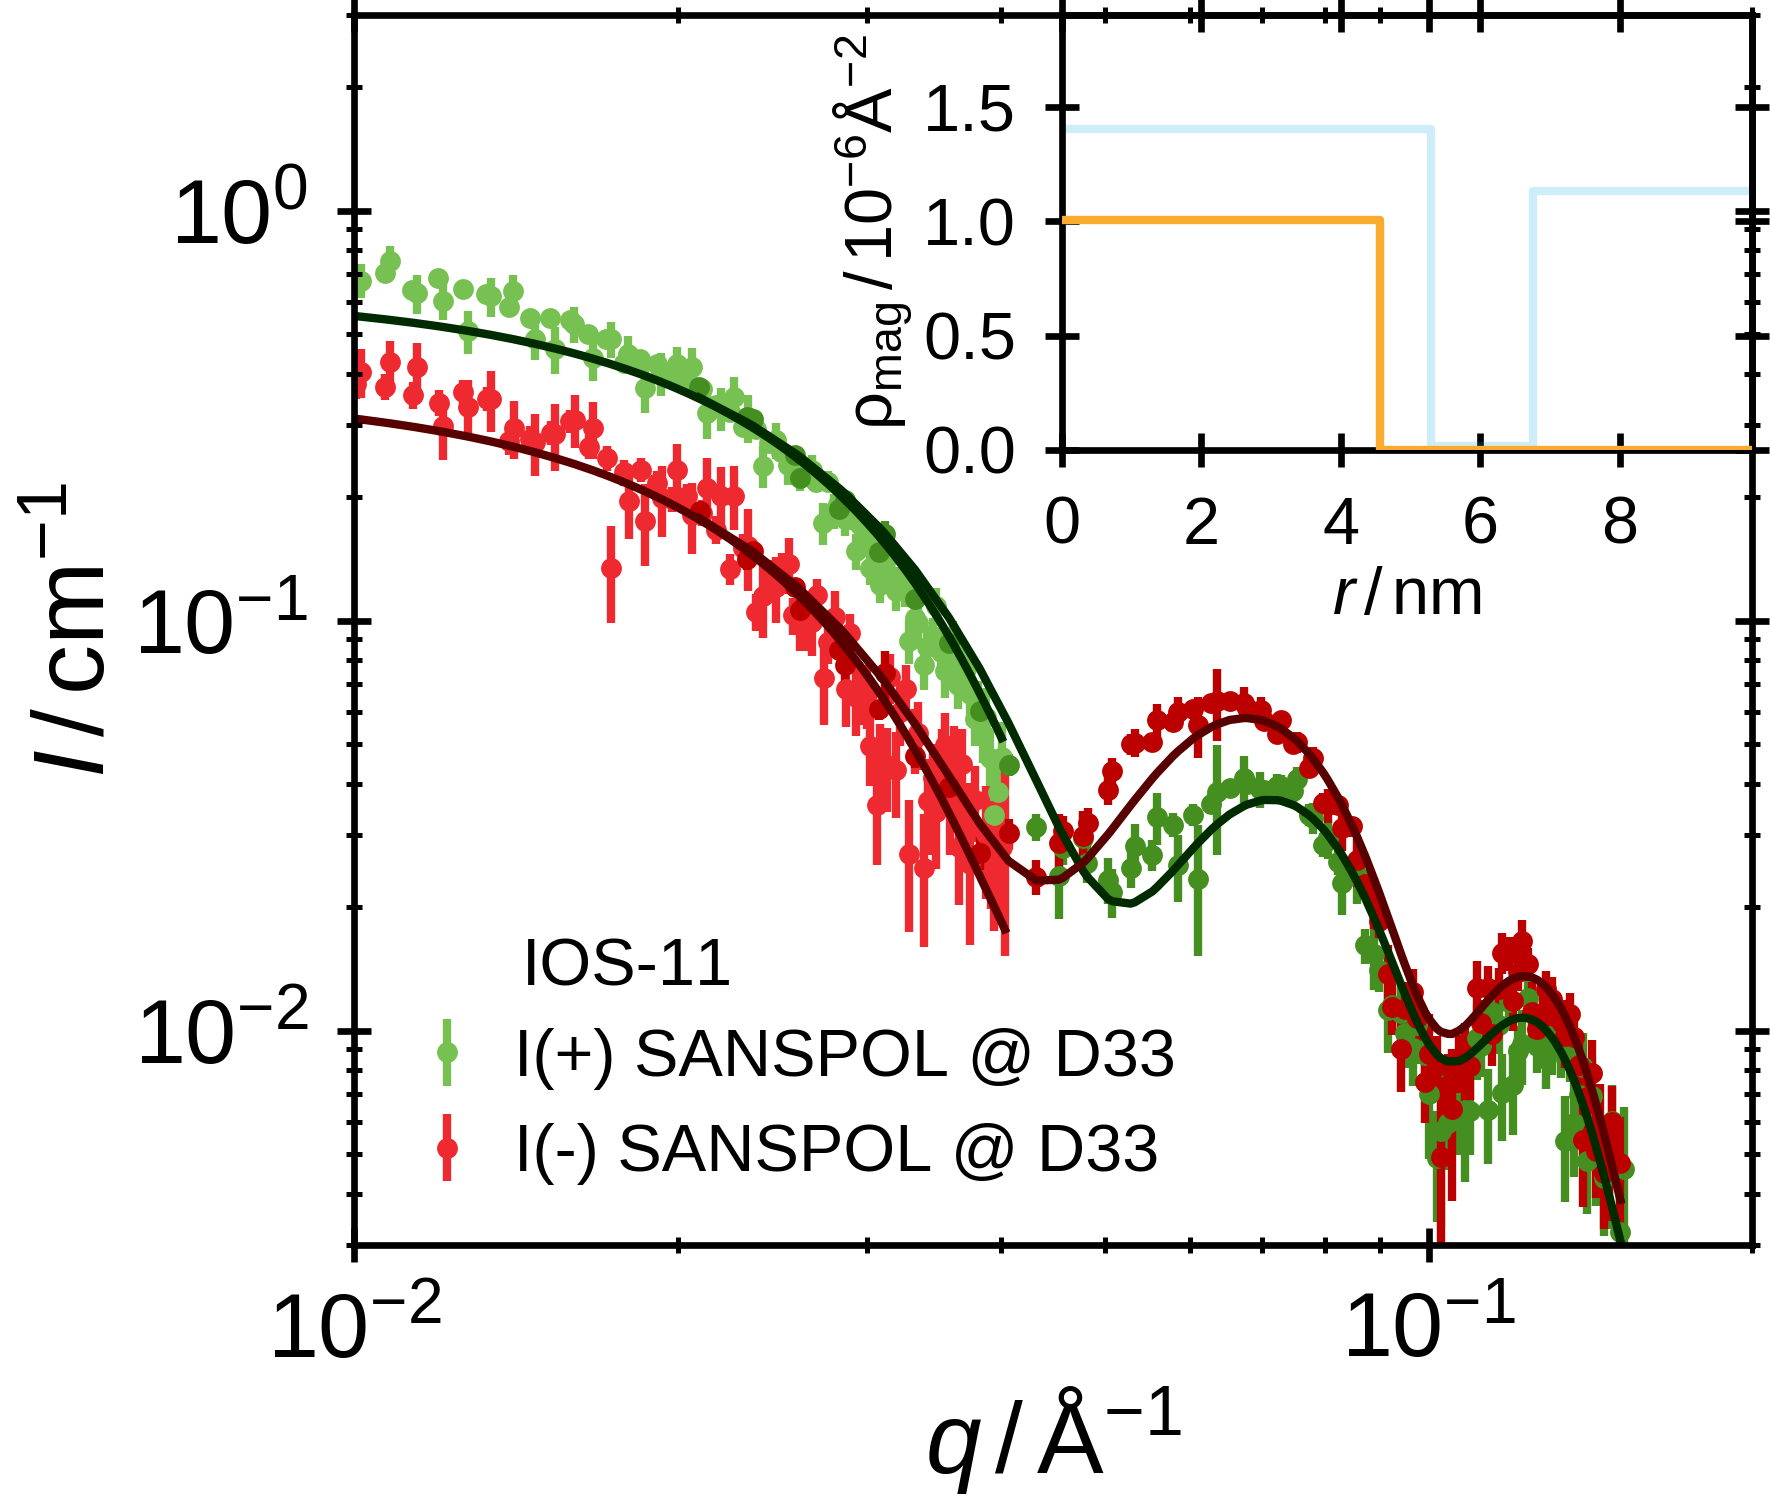
\includegraphics{looselyPackedNS_SAS_IOS-11_SANSPOL}
      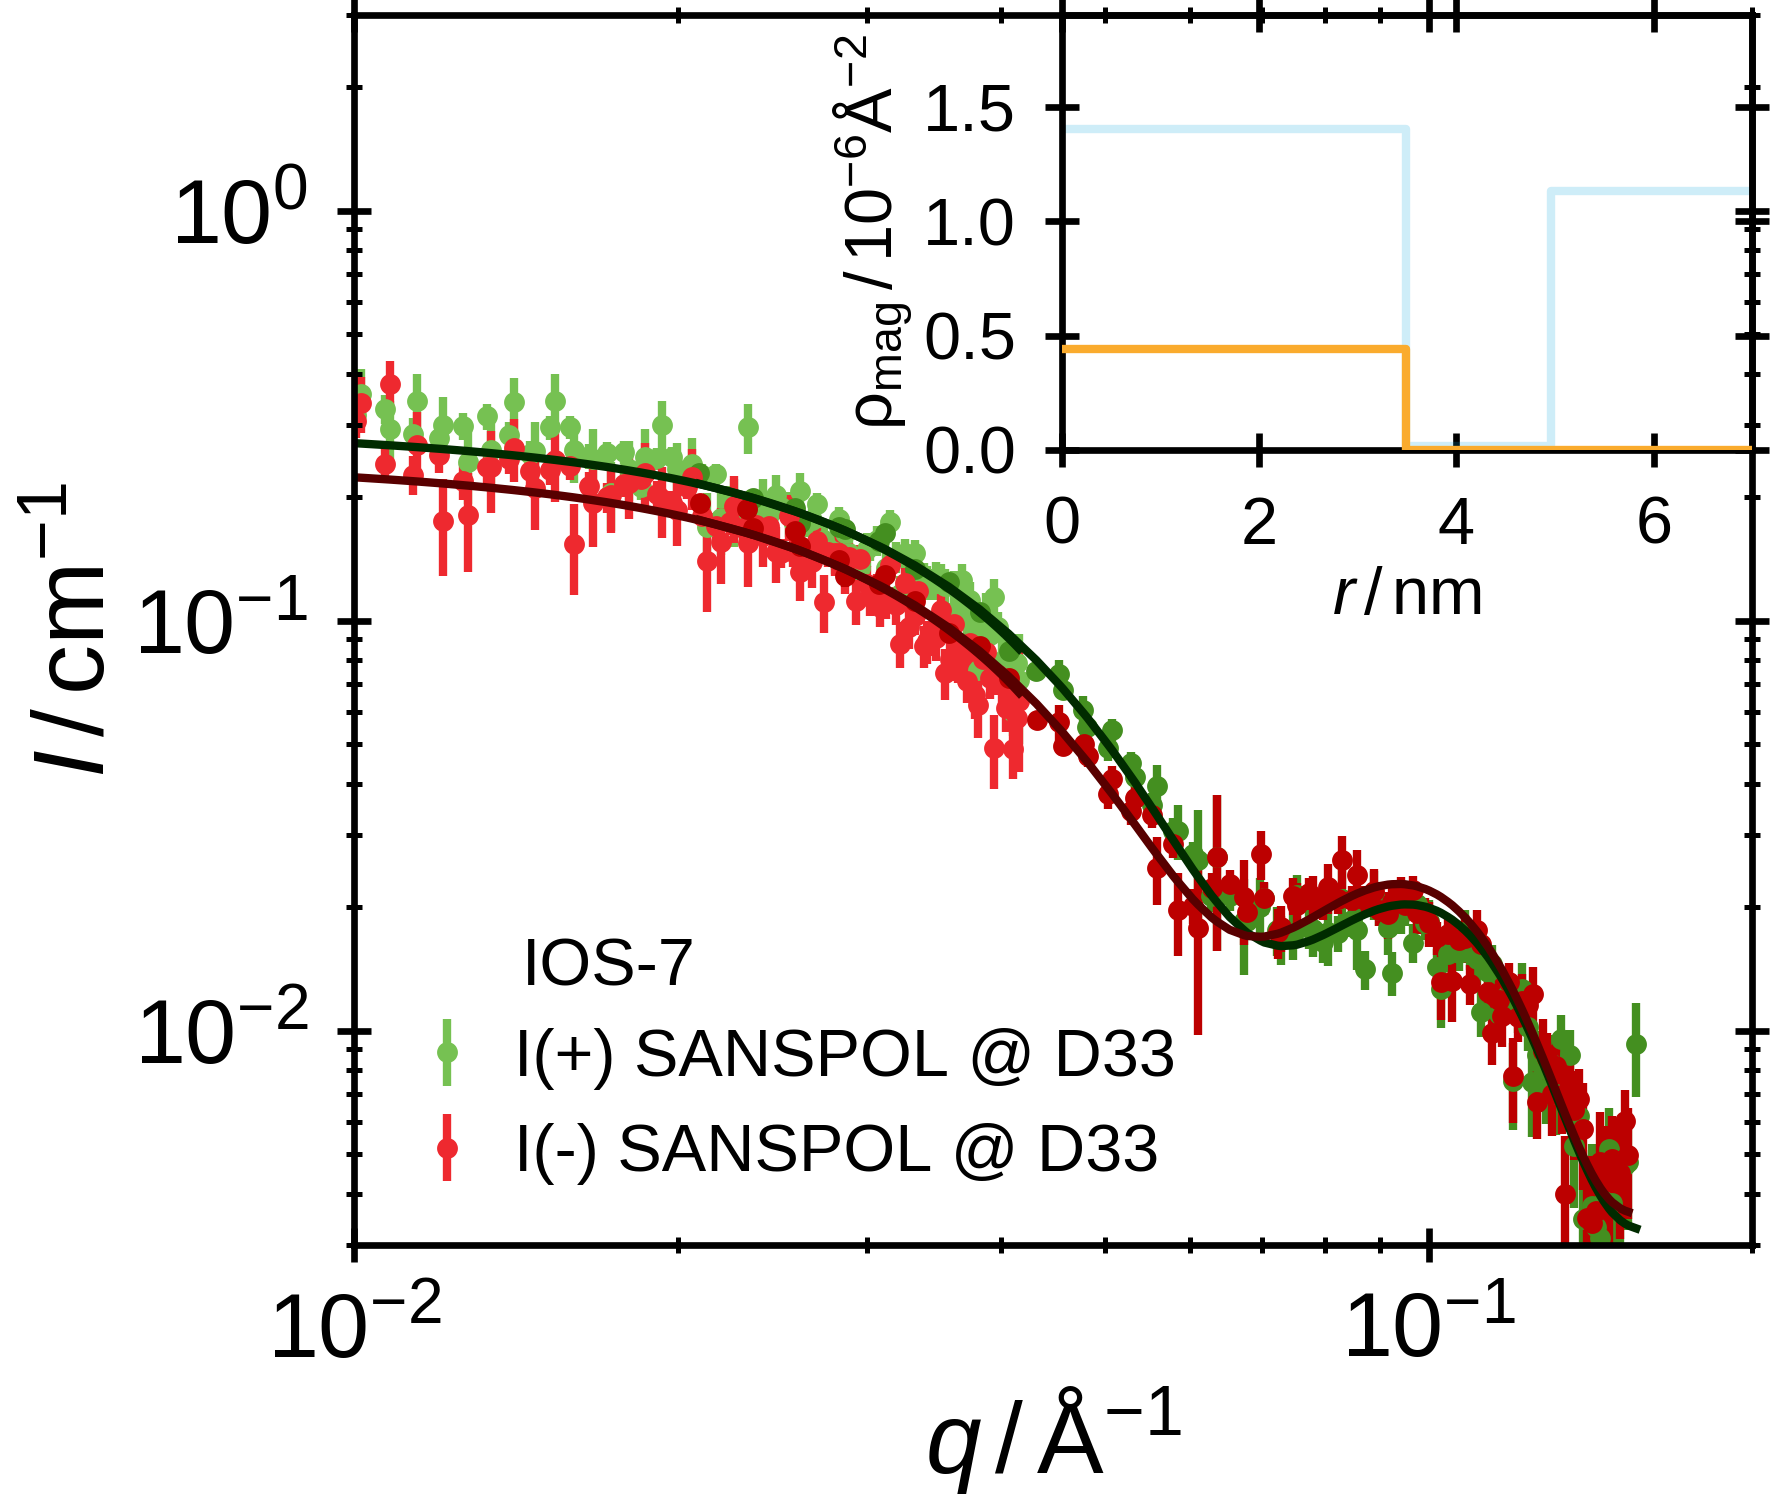
\includegraphics{looselyPackedNS_SAS_IOS-7_SANSPOL}
      \caption{\label{fig:looselyPackedNP:nanoparticle:sanspol}SANSPOL of IOS-11 (left) and IOS-7 (right) described with a spherical magnetic form factor shown in the inset, which is allowed to have a reduced size in comparison to the nuclear structure. Also shown in the inset is the nuclear form factor in blue scaled by a factor of $0.2$ for direct comparison.}
    \end{figure}

    \begin{table}[!htbp]
      \centering
      \caption{\label{tab:looselyPackedNP:nanoparticle:sanspol}Parameters for the spherical core-shell model of IOS-11 and IOS-7.}
      \begin{tabular}{ c | l | l }
        \rule{0pt}{2ex} \textbf{SANSPOL}  & \textbf{IOS-11} & \textbf{IOS-7} \\
        \hline
        \rule{0pt}{2ex} $\rho^\mathrm{mag} \, / \unit{10^{-6} \angstrom^{-2}}$ & $1.00(6)$ & $0.44(9)$\\
        \rule{0pt}{2ex} $d^\mathrm{mag. dead} \, / \unit{nm}$                  & $0.7(1)$  & $0.0(1)$\\
        \hline
        \rule{0pt}{2ex} $M_\mathrm{particle} \, / \unit{kA \, m^{-1}}$            & $344(21)$ & $151(10)$\\
        \hline
        \rule{0pt}{2ex} $\chi^2$                                               & $3.2$     & $1.6$\\
        \hline
      \end{tabular}
    \end{table}

\end{document}